\section{Data and methodology}
\label{sec:method}

The search looks for one kind of signal: an unresolved carrier at the
star's own position, narrow compared with a single correlator channel, and
drifting in sky frequency because the transmitter accelerates along the line
of sight. Over a long track its power is spread across many channels, so a
search that treats each channel on its own will miss it. The analysis
de-drifts the data before it measures them.

\subsection{The de-drifted search statistic}
\label{sec:statistic}

Each window's dynamic spectrum is stacked along every trial drift rate
$\dot\nu$. The search statistic is the largest stacked signal-to-noise
ratio anywhere on the resulting channel$\times$drift grid,
%
\begin{equation}
T(\mathbf{x})=\max_{\dot\nu,\;\nu}\;
\frac{\sum_{t} I\!\left(\mathbf{x},t,\nu+\dot\nu t\right)\big/\sigma^{2}(t,\nu)}
     {\left[\sum_{t}1\big/\sigma^{2}(t,\nu)\right]^{1/2}},
\label{eq:tstar}
\end{equation}
%
where $I(\mathbf{x},t,\nu)$ is the spectrum at sky position $\mathbf{x}$
in integration $t$ and channel $\nu$, and $\sigma(t,\nu)$ is the noise scale
there. Equation~\ref{eq:tstar} is the matched filter for a constant-drift
carrier: it adds the signal coherently along the track and divides by the
noise of the stacked spectrum, so $T$ is an absolute signal-to-noise ratio
and not a local contrast. The noise scale is the median absolute deviation
across \NCtrl{} control positions at each integration and each channel,
scaled to its Gaussian-equivalent standard deviation --- local in time and
frequency, global in position, shared by the star and every control, and with
the across-position median never subtracted from the numerator. The statistic
is evaluated at one position at a time, identically at the star and at each
control, which is what makes the two comparable. $T_\star$ denotes its value
at the star.

Spectra are extracted at the star's apparent position, never from images.
For each integration and each native channel the pipeline forms the weighted
vector average of the phase-shifted visibilities, in total intensity: the
mean $I=(XX+YY)/2$ of the two parallel-hand correlations. That average is the
dirty-map value at the extraction position --- an amplitude, not a
deconvolved flux density, so in a field with extended emission it is not a
point-source measurement. The data are used as the archive delivered them,
through ALMA's own calibration and quality assurance, with their flagging
carried through, every delivered channel searched, and no regridding,
deconvolution or edge trimming. A per-integration median along the
\emph{frequency} axis removes the continuum; no median is taken along
time, so a one- or two-channel feature cannot be removed by it. One
subtlety matters for every power quoted below: the delivered channels are
smoothed, so a channel's effective noise bandwidth is not its separation and
flux density times channel width is not yet a radiated power. A response
correction computed from the correlator's own channel shape supplies the
difference, derived and validated against the effective resolutions ALMA
reports in Appendix~\ref{app:conventions}.

One convention is fixed here and holds everywhere in the paper. The search
runs on the topocentric sky frequencies ALMA delivered, and every drift rate
quoted is the apparent one at the telescope, since that is what the data
contain and what a reader can recompute from the released channel axes. Two
steps need the star's own frame instead, and both take it: a crossing is
compared with the line catalogue, and a repeat epoch is read at the predicted
cell, after each block's frequency axis has been corrected for the Earth's
motion at that epoch and then for the star's systemic velocity. Nothing here
is evaluated in a barycentric frame alone.

Two power quantities carry the main text, both defined in
Table~\ref{tab:quantities}: the trigger level $P_{\rm trig} = 4\pi
d^{2}S\,\Delta\nu$ at distance $d$, for a carrier that makes $T_\star$ reach
$T_{\rm trig}=\StageNullTrig$ in one native channel of width $\Delta\nu$,
and the sensitivity $\mathrm{EIRP}_{90}$. The second is measured, not
assumed: synthetic carriers of known amplitude were injected into
calibrated visibilities and recovered through the unmodified pipeline,
\SelNTone{} of them over \SelNUnit{} block--window configurations of the
fine class and \SensNToneCoarse{} over \SensNInjCoarse{} of the coarse,
spanning both ALMA arrays, four bands and the sample's full range of
channel widths. Every limit quoted in
this paper is the $\mathrm{EIRP}_{90}$ of its own window, given to two
significant figures beside its native channel width; the measured
completeness is \S\ref{sec:pninetysel} and its error
budget is Table~\ref{tab:p90budget}. The absolute flux scale is checked twice from
outside, in two bands on two arrays: the extractor reproduces an
independent reduction of the same AU~Mic visibilities to
\PxJanRatio\,$\pm$\,\PxJanRatioErr, and the published quiescent flux
density of $\epsilon$~Eridani to \PxEpsRatio\,$\pm$\,\PxEpsRatioErr{}
\citep{Burton2022}.

The drift range searched is bounded by an acceleration, not by a
frequency. Drift rate and line-of-sight acceleration are one quantity in
two sets of units, $a_{\rm los}=c\,\dot\nu/\nu$, so a ceiling expressed
as $\dot\nu/\nu$ is the same physical limit in every band; the released
drift and acceleration ceilings satisfy that relation window by window, to
$\DriftRelDev$ over all \DriftRelNWin{} Class~A windows. The default
ceiling is \DriftCeilLo--\DriftCeilHi\,Hz\,s$^{-1}$\,GHz$^{-1}$, that is
$|a_{\rm los}|\le\AccelCeilMed$--$\AccelCeilMax$\,m\,s$^{-2}$. That is
the acceleration of a transmitter orbiting a solar-type star at a few
hundredths of an au. It is the \citet{Mason2025} fiducial with a
threefold margin, widened for a confirmed exoplanet host whenever the
innermost known planet demands more. It is far narrower than the general
recommendation of \citet{Sheikh2019}, which is set by solar-system
rotation and orbital motion rather than by a planet's own acceleration,
and the difference is a deliberate restriction of what this search covers
and not a weaker version of their advice. The margin is not cosmetic: at unit
margin the search would have been blind to two of the windows that
produced a crossing. The grid is uniform in $\dot\nu$, and fine enough
that a carrier midway between two trials loses no more than
\DriftGridFineHalf{} of a native channel over the longest track. Two limits
follow: the rates searched are the apparent ones at the telescope, so a
deliberately chirped carrier is not distinguished from an accelerating
platform, and a transmitter need not be bound to a known planet at all, so
drifts faster than the ceiling are simply unconstrained
(Fig.~\ref{fig:accel}).

\begin{figure}
\centering
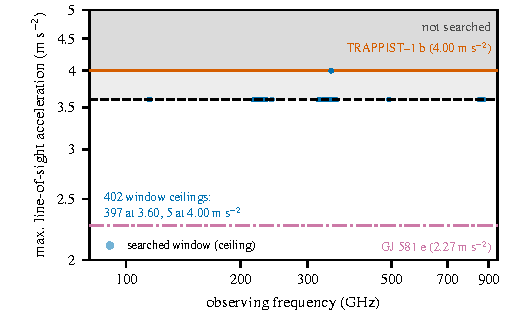
\includegraphics[width=\columnwidth]{figures/drift_acceleration.pdf}
\caption{What the drift search reaches, as a physical selection function.
The drift ceiling of each of the \NWinA{} Class~A windows (points),
converted to line-of-sight acceleration, $|a|=c\,\dot\nu/\nu$, against
observing frequency; the shaded region above is unsearched. The boundary
is flat because the grid was built at constant acceleration; in the units
the search works in it is not, running \AccelDriftLo\,kHz\,s$^{-1}$ at
\AccelFreqLo\,GHz to \AccelDriftHi\,kHz\,s$^{-1}$ at \AccelFreqHi\,GHz.
Horizontal lines are reference accelerations: Earth's rotation at the equator
(\AccelEarthRot\,m\,s$^{-2}$) and orbit (\AccelEarthOrb\,m\,s$^{-2}$), and
the two most demanding known planets of any target, \AccelWorstName{}
(\AccelWorstVal\,m\,s$^{-2}$) and \AccelSecondName{}
(\AccelSecondVal\,m\,s$^{-2}$). The boundary drawn is the default ceiling,
\AccelCeilMed\,m\,s$^{-2}$, which is also the median; it runs to
\AccelCeilMax\,m\,s$^{-2}$ on the \AccelNWide{} \AccelWideStar{} windows. For
the most demanding case, transiting TRAPPIST-1~b, \TrapPhaseHi{} per cent of
the orbital phase lies above the default ceiling and \TrapPhaseLo{} per cent
above the widened one.}
\label{fig:accel}
\end{figure}

Only part of the archive can carry a drift search at all, and the two
classes reported here are that division (Table~\ref{tab:quantities}).
Channelisation in the sample is bimodal, with an empty gap between the modes,
so the split is unambiguous, and it coincides with the physical criterion
that matters: whether the maximum searched drift crosses of order one channel
or more over the on-source track, $\eta_{\rm drift} =
|\dot\nu_{\max}|\tau_{\rm track}/\Delta\nu_{\rm ch} \gtrsim 1$. Each
window's own $\eta_{\rm drift}$, trial-drift count and acceleration ceiling
are released catalogue columns, so a reader may reclassify on that criterion
instead; the two do not partition the survey identically. \textbf{The two
classes are physically different experiments}, results are given per class,
and they are combined only where that is statistically appropriate.

\subsection{From a crossing to a confirmed signal}
\label{sec:summary}

Every window passes through the same three tests in the same order, and
three words name what comes out of them: a \emph{crossing}, an
\emph{unattributed crossing} and, had one survived, a \emph{confirmed
signal} (Fig.~\ref{fig:chain}). Each is set out below as the quantity it
measures, the number that quantity is compared with, when that number was
fixed, and what passing it does and does not establish. There is no fourth
test, and none of the three is a significance test.

\begin{enumerate}[label=(\roman*),leftmargin=1.9em,itemsep=3pt,topsep=3pt,parsep=0pt]
\item \emph{Trigger $\to$ a crossing.} The quantity is $T_\star$, the
de-drifted statistic of Eq.~\ref{eq:tstar} read at the stellar position; the
criterion is $T_\star\geq T_{\rm trig}=\StageNullTrig$ in at least one
channel$\times$drift cell; and both the statistic and the level were fixed
before the archival search began. \textbf{$T_{\rm trig}$ is a trigger
threshold and not a detection significance:} $T$ is not shown to follow any
standard distribution under the null, so the level carries no tail
probability, and a window holds between \TuCellsLo{} and $\TuCellsHi$ of
those cells, so one level buys very different protection in a coarse
single-pointing window and in a finely channelised one on a long track. A
crossing establishes only that the window goes on to the next two tests.
\item \emph{Line attribution $\to$ an unattributed crossing.} The quantity
is the crossing's velocity offset from the nearest transition of a
molecular-line catalogue, evaluated in the star's own rest frame; the
criterion is $\pm\MaskHalfKms$\,km\,s$^{-1}$. The statistic, the trigger and
the original species list were fixed before any crossing was classified; the
species list was afterwards extended, and that extension is the reason one
crossing is reported as unattributed where the list as it now stands would
attribute it (Appendix~\ref{app:linemask}). The half-width follows the Keplerian line-of-sight velocities of gas
surviving beyond a few au, with margin for the systemic velocity. A crossing
inside that window is \emph{attributed}, and the attribution is good
evidence: a coincidence with a catalogued transition makes an astrophysical
origin far more plausible than a transmitter, the more so where a second
transition of the same species or known circumstellar emission is present.
But a coincidence is a statement about a catalogue rather than a property of
a frequency, so this is an attribution and not an exclusion, and
\textbf{every crossing goes on to the recurrence test whichever side of the
window it falls}, wherever a later block covers the frequency. An unattributed crossing is a target for follow-up and not
a detection. The window's price is that the survey constrains nothing inside
it: ${\approx}\SearchedUnionGHz$\,GHz of the \UnionGHz\,GHz covered lies
outside (Appendix~\ref{app:linemask}).
\item \emph{Independent recurrence $\to$ a confirmed signal.} The quantity is
$T_\star$ at the cell the first epoch predicts, read in another execution
block of the same star at a single drift rate after the frame correction of
\S\ref{sec:statistic}; the criterion is that it reach the trigger again; and
the test was specified before the repeat epochs were searched. It is a weak
criterion, and the archive's uneven temporal sampling is why: only part of
the sample has epochs separated well enough to apply it at all.
\end{enumerate}

\emph{Two diagnostics hang off the second test, and the word is exact: each
says which crossing deserves attention first, and neither decides anything.}
The first ranks $T_\star$ against the same statistic at \NCtrl{} control
positions in the same window, drawn once from a fixed seed into an annulus
placed by each block's own synthesised and primary beams so that no control
sits on the star; its lowest value, $1/(\NCtrl+1)$, means the star beat every
control. It is a ranking filter and not a significance test, because the
stellar and control positions are not demonstrably exchangeable: out of
sample, on \HoWin{} windows the frozen pipeline had never seen, the stellar
rank has median \HoRankMed{} where one half is expected if the two were
interchangeable, and a parameter-free correction for the annulus geometry
does not restore an exchangeable statistic (Appendix~\ref{app:radius}). It
also responds to compactness rather than to origin, as $\beta$~Pictoris
shows: genuine carbon monoxide ranks below its own control ring there,
because the resolved disc lifts the ring along with the star. The second
diagnostic is a visibility-domain fit, which asks whether a crossing's
emission is at the stellar coordinates rather than elsewhere in the field; it
cannot discriminate at the trigger either, because a noise maximum at the
star has flux at the star (\S\ref{sec:vistest}). \textbf{Neither gates a
disposition, so neither is charged to the sensitivity}, and the limits here
are correspondingly deeper than a chain charging for the rank would give.
Throughout, $p$ denotes a genuine significance level, and no probability
computed against the rank's own null is called one.

\emph{One execution block is not a null, and a rule fixed in advance says so.}
The comparison with the control positions needs each block's ensemble to behave
like noise, and a block fails when the median control statistic over its own
windows, scaled by the median of that quantity over its class, exceeds
\BqFactor{} that scale. Of the \BqNBlocks{} primary-census blocks, \BqNFail{}
fails --- \BqFailBlock{} toward \BqFailStar, at \BqFailQ{} where the next worst
is \BqNextQ. \textbf{The Class~A results are identical with it and without it},
the same \BqWinACut{} windows and \BqXrossACut{} crossings either way, because
its \BqFailNWin{} windows are all coarse-channel; what it does hold is
\BqFailNCross{} of the \NCross{} crossings, the survey's entire Class~B
crossing population (Appendix~\ref{app:falsealarm}).

Because a fixed threshold is not a fixed false-alarm rate, the number of
crossings expected by chance is computed window by window, from the
exceedance rate measured at each window's own control positions; the reserved
blocks then test the one assumption that makes, which is that a star behaves
like a control position in its own field (\S\ref{sec:trigunif}).

Three corrections precede the statistic: the extraction field is chosen so
that the star lies inside the delivered primary-beam field and not merely
inside the quoted field of view; the stellar position is propagated to the
observation epoch for proper motion, though not for the annual parallax,
whose omission is corrected window by window in
\S\ref{sec:pninetysel}; and on-source time is accounted per integration
from the
delivered exposure records rather than from the scan intentions. That the
chain finds what it is meant to find is shown twice over, by the injected
carriers above and by $\beta$~Pictoris CO --- a real feature at a known
stellar position, recovered and localised in two transitions and
\NStageOneBpicEb{} execution blocks (\S\ref{sec:bpicval}).

\begin{table}
\centering
\caption{The quantities and the three words this paper uses, defined once.
Every term below is used in this sense throughout and in no other.}
\label{tab:quantities}
\small
\begin{tabular}{@{}p{0.235\columnwidth}p{0.70\columnwidth}@{}}
\hline
Term & Definition \\
\hline
Crossing &
A channel\,$\times$\,drift cell at the stellar position reaching
$T_\star\geq\StageNullTrig$. An event requiring investigation; no claimed
significance. \\
Unattributed crossing &
A crossing lying more than $\MaskHalfKms$\,km\,s$^{-1}$ in the star's frame
from every transition of the frozen line catalogue. A target for follow-up;
not a detection. \\
Confirmed signal &
An unattributed crossing recovered at the predicted stellar-frame frequency
and drift in an independent block. The only confirmation criterion. \\
$P_{\rm trig}$ &
The power of a carrier that makes $T_\star$ reach the trigger in one native
channel. An internal pipeline level: not a sensitivity, not a
significance. \\
$\mathrm{EIRP}_{90}$ &
The power at which nine injected carriers in ten are recovered at the star
through the trigger. A measured completeness, not a detection probability. \\
Class~A &
The primary experiment: \NWinA{} fine-channel windows, median
\ChanAMedKHz\,kHz, toward \NSysA{} systems over \UnionClassA\,GHz of union
bandwidth, in which the searched drift crosses of order a channel or more. \\
Class~B &
The secondary experiment: \NWinB{} coarse-channel windows, mode
\ChanBModeMHz\,MHz, constraining a persistent unresolved excess. No drift
discrimination, and never a carrier search. \\
The sample &
Neither volume-limited nor representative of the solar neighbourhood: the
stars ALMA happened to observe for other reasons (\S\ref{sec:sample}). \\
\hline
\end{tabular}
\end{table}

%% HANDOVER (04_method.tex, round 11, r11-chain) -- supersedes the round-10 note.
%% THE CHAIN IS NOW THREE STEPS: trigger -> line attribution -> recurrence.
%%   The rank and the visibility fit are diagnostics attached to the SECOND
%%   step and gate nothing, so nothing in this paper may charge their cost to
%%   a sensitivity, and the word "candidate" is no longer a defined term
%%   anywhere: the three words are crossing / unattributed crossing /
%%   confirmed signal.
%% tab:quantities IS NOW IN THIS FILE and is the single definition of all
%%   eight terms (R1-10).  It is what licenses the deletion of the repeated
%%   caveats elsewhere; the list of repetitions it pays for is entry 7 of
%%   /workspace/SETI/referee_r11/INTEGRATION_QUEUE.md.
%% DELETED to pay for it: the whole of old stage (iii) (the spatial screen as
%%   a gate, 37 lines), the two-stratum EIRP90 sentences, the screen-cost
%%   arithmetic, and the free-standing visibility-check and rank-displacement
%%   paragraphs, both folded into the diagnostics paragraph.
%% STILL OPEN, queued in /workspace/SETI/referee_r11/INTEGRATION_QUEUE.md:
%%  * fig:chain prints as Figure 8 but is first cited here; the float lives in
%%    05_results.tex.  Either file may host it, but it must be renumbered or
%%    moved.
%%  * the third correction below still says the stellar position is
%%    "propagated to the observation epoch".  It becomes "proper motion and
%%    annual parallax both" the moment r11-sens's re-extraction lands (M5),
%%    and not before -- we must not assert a correction we have not applied.
%%  * no Class A EIRP90 multiplier is quoted here ANY MORE, deliberately: one
%%    adopted figure belongs in S5.1 and Table 4 and nowhere else.
%% NUMBERS STILL WANTED here: a macro for the Keplerian half-width (the typed
%%   13 km/s is gone from stage (ii), and so is the figure) and one for the
%%   threefold drift margin.
%% Table 10 (tab:algorithm) in App A remains unreferenced -- its citations
%%   were here and the three-step chain replaces it; the appendix owner should
%%   delete the float.
